\documentclass[12pt, oneside]{article}   	% use "amsart" instead of "article" for AMSLaTeX format
\usepackage[margin=1in]{geometry}                		% See geometry.pdf to learn the layout options. There are lots.
%\usepackage{cite}
\geometry{letterpaper}                   		% ... or a4paper or a5paper or ... 
\usepackage{graphicx}				% Use pdf, png, jpg, or eps§ with pdflatex; use eps in DVI mode
								% TeX will automatically convert eps --> pdf in pdflatex
\usepackage{titling}		
\usepackage{amssymb}
\usepackage{url}
\usepackage{titlesec}
\usepackage{booktabs}

\titleformat{\section}
  {\normalfont\fontsize{15}{15}\bfseries}{\thesection}{1em}{}
\titleformat{\subsection}  {\normalfont\fontsize{12}{15}\bfseries}{\thesubsection}{1em}{}

\setlength{\droptitle}{-5em}
%\setlength{\dropauthor}{-3em}

\pretitle{\begin{center} \Large}
\title{Predicting Henry's Law Using Chemical Structure with Graph Convolutional Neural Networks}
\posttitle{\end{center} \lineskip 0.1em}
\preauthor{\begin{center} 
	\large \lineskip 0.1em}
\author{Zach Calhoun}
\postauthor{\par\end{center} \lineskip 0.5em}
\predate{\begin{center}\large}
\postdate{\par\end{center}}
%\date{}	

\begin{document}

\maketitle
%TODO - match formatting laid out in project description

\section{Abstract}
Henry's law, or the air/water partitioning coefficient, refers to ratio of how a given chemical compound partitions between air and water at equilibrium. Obtaining measured values for this ratio is difficult, so environmental chemists often rely on regression models to understand partitioning behavior. These models generally take one of two approaches: they use known physiochemical properties, or they use the chemical structure itself. The first method, while often more accurate, depends on having measured properties a priori. For poorly studied compounds, this method may not be feasible, making the ability to predict on structure alone more important. In this article I explore how existing methods based on structure may be improved using Graph Convolutional Neural Networks (GCNNs). Using this method I achieved a test set performance ($R^2=0.895$) on par with a Random Forest model that used physiochemical properties ($R^2=0.894$). This performance came close to the prediction performance achieved using the Environmental Protection Agency's OPERA model, which also uses physiochemical properties ($R^2 = 0.905$). This finding demonstrates the usefulness of applying Graph Neural Networks to the application area of environmental toxicology when assessing the environmental risk of new compounds.

\section{Problem Statement}
Roughly 10 million new chemicals are synthesized each year, and the EPA is only equipped to screen a fraction of these chemicals for environmental risk \cite{burton}. Of particular concern are so-called PBT (persistent, bioaccumulative, and toxic) chemicals. These chemicals are unique because they do not break down, they are particularly toxic, and because they bioaccumulate, they risk making their way into the food chain \cite{matthies}.

Perhaps the most infamous example of a PBT is DDT, the fertilizer used during the 20th century that was found to be highly toxic to bird populations, inspiring Rachel Carson's \emph{Silent Spring}. The more recent example making headlines today is PFAS (per-fluorinated alkyl substances), which represents the class of chemicals commonly found in non-stick pans or in water-repellant clothing. In both cases, the chemicals were synthesized for a particular purpose, and the risk to society was discovered decades later. Decades later, however, is far too late. Both PFAS and DDT are now ubiquitous, found in remote locations such as the Arctic, as well as in a large percentage of the population's bloodstream \cite{czub}.

To prevent this pattern from repeating itself, the EPA conducts environmental risk assessments using known and estimated chemical properties to predict chemical fate and toxicity in the environment. However, the EPA can only  study a fraction of the compounds they need to, and estimations can be unreliable, especially when the chemical's properties are poorly understood \cite{burton}. When there are few or no physiochemical properties measured, estimates rely on structure alone. The Bond Contribution Method is one such method, used for measuring Henry's law \cite{meylan}. This method is based on a small set of chemicals, and its output may be unreliable, since it only focuses on the bonds in the molecule rather than the structure as a whole. 

If we could better predict environmental fate using structure, then environmental chemists could more accurately assess the true risk of new compounds on the market, allowing society to better prevent the widespread adoption of chemicals that pose significant environmental threats.

\section{Data Summary}
Henry's law is a well studied partitioning coefficient, meaning a lot of chemicals have values based on observations rather than estimations. For this project, I searched for a dataset that provided the Henry's law constant in a standardized format. That is, the values given for the constant need to have consistent units, be taken at standard temperature and pressure, and clearly indicate the source of the measurement, as it is vital that models are trained on observed values, rather than calculated values. 

\subsection{Henry's Law Constants}
I found a compilation of Henry's law constants in \cite{sander2015}. This compilation contains over 17,000 values for over 4,600 chemicals. Each chemical had several values given, with sources including actual measurements, and a variety of estimation methods (e.g., a thermodynamical calculation can be used to predict Henry's law). 

The author of this compilation provided the data through the webpage cited in \cite{sander-website}. Since the data was provided as a large SQL query, I ran the query using PostgreSQL to construct the tables needed to extract the data. I then selected all columns from  the \texttt{henry} table joined with the \texttt{species} table so that I could see a list of Henry's law values for each compound. This query was saved into a CSV file so that analysis could be done outside of SQL.

\subsection{Chemical Properties}
While the source mentioned above provided the Henry's law constants, this source did not provide the chemical properties needed to build a model. Most notably, many examples of predicting chemical properties from structure in machine learning make use of the Canonical SMILES (Simplified Molecular Input Line Entry System) representation of the chemical. The SMILES representation is a string representation of the chemical from which one can determine both the atoms comprising the molecule as well as the structure of the molecule, with the Canonical flavor of SMILES referencing the fact that each compound's SMILES representation is unique \cite{oboyle2012}.

To get this representation for each molecule, I used the package PubChemPy \cite{PubChemPy}. This open-source project is a package that accesses PubChem, an online search tool for obtaining chemical information, using PubChem's Power User Gateway \cite{kim2015}. This data source is assumed reliable since it is managed by the National Institute of Health, and the open source package is merely a convenient method for accessing this data.

Additionally, the package DeepChem was used to extract chemical descriptors for each of the molecules. This list of descriptions includes properties such as number of hydrogen donors / acceptors and number of valence electrons, as well as structural information about the chemical groups present (e.g., whether there is an amine group present in the molecule) \cite{Ramsundar-et-al-2019}. This package is built on top of RDKit, an open source toolkit for cheminformatics \cite{rdkit}.

\section{Preprocessing the data}
Given that there was one primary dataset, and an auxiliary dataset to fill in gaps, significant preprocessing was required to complete the dataset.

\subsection{Joining the Data}
First, the compilation of Henry's law constants was reduced to unique compounds with measured values. There were two values for two compounds, so the measurements were averaged to ensure one measured value per compound. Following this reduction, there were 1,025 compounds left over.

For each compound, PubChem was queried to get further information using the chemical's unique identifier (the Inchikey), which the compilation contained as a unique reference. For the 1,025 compounds, only those with 1 unique match in the PubChem database were kept. This resulted in a dataset containing 960 compounds. Individual elements in this list were discarded, as these elements do not contain bond information, and thus could not be used in the models. Lastly, chemical subcategories were reviewed to ensure adequate representation of compounds. These subcategories refer to the unique chemical groups used by chemists to classify compounds. Example subcategories include alcohols (chemicals with OH substituents) or alkanes (simple carbon chains). Chemicals in subcategories with less than 5 examples were removed, so that the model's performance could be generalized across subcategories. This resulted in a final dataset of 933 unique compounds, representing 46 subcategories. 

\subsection{Log Transform}
Values for Henry's law fall in the range of 0 to infinity. If the value is zero, the compound may vaporize almost immediately out of its aqueous phase into the atmosphere, and an infinite value indicates that the compound strongly prefers the aqueous phase. I use the term infinite here to indicate the theoretical limit, but in practice, a strongly hydrophilic, or water-loving, compound will have a very large constant. In this dataset, the range of observed values is $(1.2\times10^{-7}, 2.3\times 10^{10})$. To address this large difference, I performed a log-transform on the Henry's law values. This makes sense from a practical point of view; environmental engineers often care about the order of magnitude rather than the actual value when calculating Henry's law. The distribution of the log-transformed data is approximately normal, representing a relatively balanced dataset, as shown in the supplementary material.

\section{Methods}
To model and predict chemical behavior, there are generally two schools of thought: use physiochemical descriptors to create a tabular representation of a molecule, or use the actual structure itself \cite{Ramsundar-et-al-2019}. Using just the structure itself is difficult, as unique representations of the molecule must be formed, and for a set of molecules, the model must be able to assess compounds with varying numbers of bonds and atoms. Historically, computational toxicologists have relied on algorithms that generate unique fingerprints for each molecule. These fingerprints can then be truncated so that each molecule has a representation with similar dimensions. However, graph neural networks have recently unencumbered computational toxicologists from requiring such fingerprints. To understand the efficacy of graph neural networks in the context of predicting Henry's Law, I created one model using physiochemical properties and one model using graph neural networks.

To compare performance across models, I split the data into an 80\%/20\% train and test set, with hyperparameter tuning done using cross validation within the training set. Additionally, since the goal of each model is regression, I computed the $R^2$ value and the Mean Squared Error (MSE) on the training and test sets for each model. 

\subsection{Using Physiochemical Properties}
Using the SMILES representation, the RDKit Feature Descriptors were queried to get a representation of the molecule containing 208 physiochemical properties. This list contained descriptors such as molecular weight and number of valence electrons, but also properties such as ring count, which means that this data contains some information about the structure beyond physiochemical properties. Since the goal of this section is to provide a baseline using simpler representations of the molecules, this data was kept.

Because this dataset is tabular, several models were initially attempted using SciKit Learn, since this package enables the quick training and evaluation of model performance \cite{scikit-learn}. Models considered included a Random Forest Regressor, Ridge Regression, and K-Nearest Neighbors Regression. The highest $R^2$ value was achieved using the Random Forest Regressor with its default settings ($R^2=0.87$), whereas Ridge Regression and K-Nearest Neighbors Regression did not exceed $R^2= 0.81$ and $R^2=0.61$, respectively, under a variety of hyperparameter settings.

Random forest regression learns to model by generating an ensemble of decision trees, where each decision tree is given only a subset of the features. Each decision tree is generated by splitting the data based off of which feature split most decreases MSE. The random forest model then averages the predictions from each decision tree for its output. Given that the feature set is sparse for each compound, with only a subset of features being important within each subcategory, it makes sense that this model excels. Within the entire set of compounds, there are a few features that explain the variance, but within each subcategory, another set of features explain the variance within that subcategory. This is demonstrated in the supplemental material using principal components analysis, and it also demonstrates why dimensionality reduction attempts failed to improve model performance.

In a Random Forest model, several hyper parameters my be tuned to improve performance. The number of decision trees used can be increased to include more permutations of the features and data, and overfitting can be prevented by constraining the learned trees to have a smaller max depth. Several values were considered to determine the optimal parameters by performing 4-fold cross validation on the training set, so that the validation set would be about the same size as the test set. The optimal number of decision trees wound up being 200, with an optimal max depth of 10.

\subsection{Using a Graph Neural Network}
	A Graph Convolutional Neural Network (GCNN) was chosen because of its ease of implementation using the DeepChem library. Other models considered were Graph Attention Networks and Message Passing Neural Networks, again because of their ease of implementation \cite{Velickovic2017, Gilmer2017}. However, the Graph Convolutional Neural Network initially demonstrated the best performance with the lowest gap between the validation and test set $R^2$ values, suggesting an already well-tuned model resistant to overfitting. Additionally, this model trained much quicker than the alternatives, so focus was spent on further refining this model to determine whether additional improvements could be made.

	This implementation of a GCNN is based on the paper by \cite{Kipf2016}. The general idea behind this model is represented by equation~\ref{eqn:gnn}. 
\begin{equation}\label{eqn:gnn}
H^{l+1} = \sigma(\tilde{D}^{-1/2}\tilde{A}\tilde{D}^{-1/2}H^{l}W^l)
\end{equation}
In this equation, the adjacency matrix $\tilde{A}$ represents the undirected graph structure. This representation is a matrix in $\mathbb{R^{N\times N}}$, where $N$ is the number of nodes in the graph. The $ij$th value in this matrix indicates whether node $i$ and node $j$ are connected. $\tilde{D}$ represents a normalization factor, used to prevent exploding or vanishing gradients. $H$ represents the previous hidden output (or the original input, $X$), and $W$ are the weights to be learned. Thus, information is passed between nodes at each layer to create new representations for each node. By repeating this process multiple times, the model learns complex relationships between distant nodes. To produce the predicted regression value, two vectors are concatenated and fed into a multi-layer perceptron (MLP). The first vector in this concatenation contains weighted and summed values from the final hidden layer output, and the second vector is the max pooling output \cite{gcnmodel}.

	To feed the Henry's Law dataset into this model, the SMILES representation for each compound was used as the input to DeepChem's \emph{MolGraphConvFeaturizer}, which is based on \cite{Kearnes2016}. In this representation, each atom in the compound is represented as a 30-dimensional feature vector comprised of the atom type as a one-hot vector, formal charge, hybridization as a one-hot vector of \emph{sp, sp2} or \emph{sp3}, aromatic (boolean), a one-hot vector of the degree of the atom, a one-hot vector containing the number of hydrogen atoms connected to the atom, chirality (boolean), and partial charge.
	

\subsubsection{Training the GCNN}
	Due to the time it takes to train a model, rather than review parameters using cross-validation, the data held out for training was again split into an 80/20 training / validation split.
	
	In the DeepChem implementation of a Graph Neural Network, the model allows for the addition of a dropout parameter for the output of each GCN layer, a drop out parameter in the final MLP layer, and the use of an activation function. The dropout parameter selects nodes with probability $p$ to turn off during one epoch, so that the model does not perform back-propagation on those nodes, with the goal of preventing overfitting \cite{Srivastava2014}. Only the addition of a drop out parameter in the MLP was found to improve performance. Several values were tested, but a value of $p=0.2$ was found to result in the most robust model, with both the best performance on the test set with the lowest difference between the training set and the test set over 70 epochs, as demonstrated in Figure~\ref{fig:traintest}.
	
\begin{figure}[!h] %  figure placement: here, top, bottom, or page
   \centering
   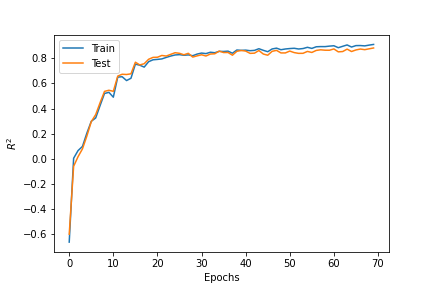
\includegraphics[width=4in]{traintest.png} 
   \caption{Train and Test $R^2$ over 70 epochs. Results suggest little overfitting.}
   \label{fig:traintest}
\end{figure}

A ReLU activation function was considered, but surprisingly, validation performance slightly dropped, so no activation function was used for the output of each GCN layer \cite{Agarap2018}. Being a neural network, this model could be tuned further by changing the network structure, but since the model reached similar performance levels to the Random Forest model, improvements are left as future work.

The final performance was evaluated on a model trained on the complete training set. Upon training the code multiple times, it was found that there were several alternate solutions found, so the best performance was reported. This likely occurred because local minimums in the model were discovered. For training, the Adam optimizer was used with a learning rate of 0.001, using the L2 loss function \cite{kingma2014}. Optimal solutions were found in 70 epochs, and training time on a CPU took 1-2 minutes. 

\section{Results}
% Treat this as a discussion...
A summary of model performance is provided in Table~\ref{tab:results}. The GCNN and the RF both performed similarly on the test set, with performance on the training set suggesting that the RF model overfit in comparison. For context, the results for the OPERA model are provided \cite{Mansouri2018}. This model was chosen for comparison because this model provides the predictions on the EPA's CompTox Dashboard \cite{williams2017}.  This dashboard contains a suite of tools developed by the US EPA to help researchers assess chemicals for health and environmental risks, and thus provides a benchmark of the utility of the models tested in this paper.

	Performance for both the RF and GCNN models was slightly worse on the same test set than the OPERA model. However, when assessed over all chemicals used in this study, OPERA's performance is significantly worse. This suggests that more validation is needed to compare the models presented. Overall performance can be better assessed by using cross-validation to get a set of train/test $R^2$ and MSE values for each of the models, which can be averaged as a whole. Additionally, performance within chemical categories should be assessed to determine whether the GCNN may present benefits over the OPERA model for specific categories. Lastly, it is unclear whether outputs from the OPERA model may indeed include measured Henry's law constants rather than predictions, since one of the physiochemical properties listed in the project includes the Henry's law value itself \cite{Mansouri2018}. 

% Requires the booktabs if the memoir class is not being used
\begin{table}[!h]
   \centering
   %\topcaption{Table captions are better up top} % requires the topcapt package
   \begin{tabular}{c c c c c} % Column formatting, @{} suppresses leading/trailing space
      \toprule
      Model    & Train $R^2$ & Test $R^2$ & Train MSE & Test MSE \\
      \midrule
      RF    & 0.967 & 0.894 & 0.126 & 0.431 \\
      GCNN & 0.935 & 0.895 & 0.244 & 0.425 \\
      OPERA (same test set) & - & 0.905 & - & 0.388 \\
      OPERA (whole dataset) & - & 0.725 & - & 1.03 \\
      \bottomrule
   \end{tabular}
   \caption{Results shown for the RF and GCNN. MSE and $R^2$ are computed on both the same test set for the OPERA method, as well as for all chemicals analyzed.}
   \label{tab:results}
\end{table}

Given this context, the performance of the GCNN demonstrates that chemical structure alone can predict Henry's law with near equal accuracy to models based on physiochemical properties. This performance suggests that this method can be used to assess novel chemicals, for which its physiochemical properties may not be measured.

To my knowledge, this is the first example using a graph neural network to predict Henry's law on measured data using only the structure itself. A previous attempt at applying a GCNN to this problem used Henry's Law values based on sorption theory within a limited domain (Metal-Organic Frameworks) \cite{zhang2021}. Additionally, highly accurate models ($R^2$=0.99) have been created using physiochemical properties \cite{English2001}. However, the OPERA model is preferred because of its adherence to OECD guidelines for valid Quantitative Structure-Activity Relationship models \cite{oecd2014}. Namely, interpretable models are preferred.

\section{Conclusions}
This study demonstrates that GCNNs can be successfully applied to predict Henry's Law with comparably high accuracy. The applicability of this model is limited to poorly studied chemicals for which standard models may not predict well. More thorough validation of performance is suggested to confirm results and evaluate how compound subcategory performance compares between this model and the OPERA model used by the EPA. Further research should explore improving this model so higher performance can be reached, and on its interpretability so that it may be accepted by the chemistry community as a useful tool.

\newpage

\bibliography{ds4cee-final-project}{}
\bibliographystyle{ieeetr}


\newpage
\section{Broader Impacts}
The United States Environmental Protection Agency cannot keep up with assessing the ecotoxicological risk of the vast number of new chemicals produced each year, prompting calls for external research \cite{burton}. Additionally, machine learning applications are biased towards problems like drug discovery, leaving a gap in the field of environmental chemistry. This paper shows that environmental chemistry could benefit from the further application of machine learning methods, and that machine learning could help the US EPA more rapidly and accurately assess the environmental risk of new compounds on the market. The OECD's requirement of interpretability poses an additional challenge to applying models in this field. Hopefully, this requirement will motivate machine learning researchers to better understand why graph neural networks can predict chemical properties well, with the benefit of helping chemists to better understand their field, too. This goal of better prediction and better interpretability will help scientists to better understand what makes a chemical particularly risky, and with this improved understanding, perhaps legislation could be applied so that the precautionary principle is taken when chemicals match this risk profile. This would obviate the EPA's current methodology of trying to keep up with new compounds on the market by preventing those chemicals from reaching the market in the first place, thus saving time and resources while conserving environmental and human health.


% Supplementary material goes here.
\newpage
\section{Supplemental Material}
\subsection{Distribution of the Data}
The distribution of the log-transformed data is shown in Figure~\ref{fig:dist}. This distribution is roughly balanced in that there is approximately equal representation of extreme values. However, the right tail of $K_H$ shows that there are higher extremes for larger $K_H$ values. In practice, these higher extremes represent molecules that are more likely to be found in the aqueous phase than in the vapor phase. 

\begin{figure}[h!] %  figure placement: here, top, bottom, or page
   \centering
   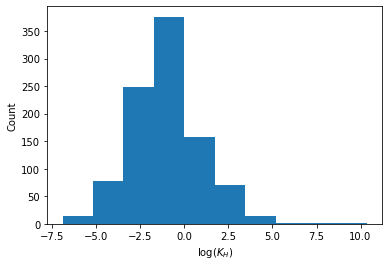
\includegraphics[width=4in]{data-dist.png} 
   \caption{The Distribution of $\log K_H$, where $K_H$ refers to the Henry's Law Constant.}
   \label{fig:dist}
\end{figure}

\newpage
\subsection{Analysis of Principal Components}
To analyze how the data using physiochemical properties varies, Principal Component Analysis was used. When graphing the data into the first two principal components, for all subcategories, the first principal component explains only a small number of molecules, with most of the variance along principal component 2, as shown in Figure~\ref{fig:pc1}.

\begin{figure}[!h] %  figure placement: here, top, bottom, or page
   \centering
   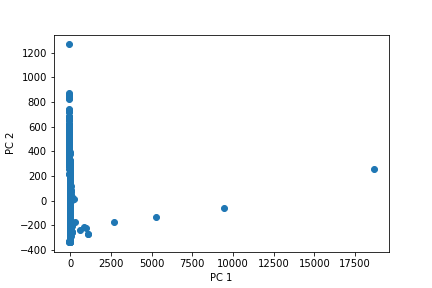
\includegraphics[width=4in]{PCA_all.png} 
   \caption{Principal Components for all of the data}
   \label{fig:pc1}
\end{figure}

However, if we look at the principal components within a specific subcategory, as shown in Figure~\ref{fig:pc2}, we see that the principal components look drastically different, with the molecules within the subcategory (labelled subcategory 40) demonstrating uniformity, and a potential third principal component explaining a large portion of the remaining variance.

\begin{figure}[!h] %  figure placement: here, top, bottom, or page
   \centering
   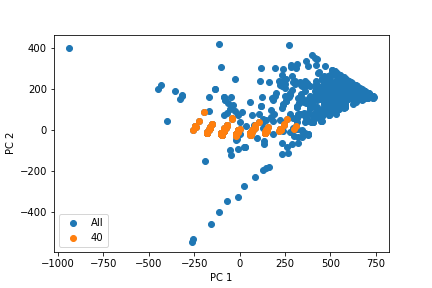
\includegraphics[width=4in]{PCA_subcat40.png} 
   \caption{Mapping data into the principal components for one subcategory}
   \label{fig:pc2}
\end{figure}

This suggests that the components that explains the variance in one subcategory does not explain the variance of the data as a whole. 

\section{Honor Code}
I adhered to the Duke honor code.

\emph{Zachary D Calhoun}

\end{document}  